\documentclass[12pt]{article}
\usepackage{preamble}

\pagestyle{fancy}
\fancyhead[LO,LE]{$\mathcal{D}$искретная математика}
\fancyhead[RO,RE]{Лекции Чухарева К. И.}

\renewcommand{\thesection}{}

\begin{document}

    \tableofcontents
    \clearpage

        % begin dismath_2024_04_23.tex

    \section{7. Комбинаторика}

    \textbf{Базовые понятия:}

    \begin{itemize}
        \item \textbf{Алфавит} (Alphabet) $\Sigma$ (или $X$, \Exs $X = \Set{a, b, c}$) - множество символов в нашей системе

        \vspace{5mm}

        \item \textbf{Диапазон} (Range) $[n] = \Set{1, \dots, n}$ - конечное множество последовательных натуральных чисел

        \vspace{5mm}

        \item \textbf{Расстановка} (Ordered arrangement) - последовательность каких-либо элементов (тоже самое, что кортеж),
        \Exs $x = (a, b, c, d, b, b, c) \quad |x| = n$

        Расстановку можно представить как функцию $f : \underset{\text{domain}}{\undergroup{[n]}} \to \underset{\text{codomain}}{\undergroup{\Sigma}}$, которая по порядковому номеру выдает символ

        $ran f = \Set{c \in \Sigma \ | \ \exists i \in [n]\ :\ f(i) = c}$

        \vspace{5mm}

        \item \textbf{Перестановка} (Permutation) - $\pi : [n] \to \Sigma$, где $n = |\Sigma|$

        Расстановка $\pi$ - биекция между $[n]$ и $\Sigma$

        \Ex $\pi = \mathtt{2713546}$

        \vspace{3mm}

        \begin{tabular}{l|ccccccc}
            i      & 1          & 2          & 3          & 4          & 5          & 6          & 7          \\
            \hline
            \pi(i) & \mathtt{2} & \mathtt{7} & \mathtt{1} & \mathtt{3} & \mathtt{5} & \mathtt{4} & \mathtt{6}
        \end{tabular}

        \vspace{5mm}

        \underline{Одна из задач комбинаторики} - посчитать количество различных расстановок или перестановок при заданных $n$ и $\Sigma$

        \vspace{5mm}

        \item \textbf{$k$-перестановка} (k-permutation) - расстановка из $k$ различных элементов из $\Sigma$

        \Ex $\underset{\text{5-perm из } \Sigma = [7]}{\undergroup{|31475|}} = 5$

        $k$-перестановка - инъекция $\pi : [k] \to \Sigma$ ($k \leq n = |\Sigma|$)

        \vspace{5mm}

        \item $P(n, k)$ - множество всех $k$-перестановок алфавита $\Sigma = [n]$ (если исходный алфавит не состоит из чисел, то мы можем сделать биекцию между ним и $[n]$)

        $P(n, k) = \Set{f \ | \ f : [k] \to [n]}$

        Чаще интересует не само множество, а его размер, поэтому под обозначением $P(n, k)$ подразумевается $|P(n, k)|$

        \vspace{5mm}

        \item $S_n = P_n = P(n, n)$ - множество всех перестановок. Также чаще всего нас будет интересовать не множество, а его размер

        $|S_n| = n!$ - всего существует $n!$ перестановок

        $|P(n, k)| = n \cdot (n - 1) \cdot (n - 2) \cdot \dots \cdot (n - k + 1) = \frac{n!}{(n - k)!}$

        \vspace{5mm}

        \item \textbf{Циклические $k$-перестановки} (Circular $k$-permutations)

        $\pi_1, \pi_2 \in P(n, k)$ - циклически эквивалентны тогда и только тогда:

        $\exists s \ | \ \forall i \ \pi_1((i + s) \% k) = \pi_2(i)$


        \Ex $\pi_1 = \mathtt{76123}, \pi_2 = \mathtt{12376}$

        \begin{tikzpicture}
        \node[circle, draw=black!60, thick, minimum size=0.5cm] (s00) {\mathtt{7}};
        \node[below=1cm of s00] (pi1) {$\pi_1$};
        \node[below left=0.66cm and 1cm of s00] (s01) {\mathtt{6}};
        \node[below right=1cm and 0.13cm of s01] (s02) {\mathtt{1}};
        \node[below right=0.66cm and 1cm of s00] (s04) {\mathtt{3}};
        \node[below left=1cm and 0.13cm of s04] (s03) {\mathtt{2}};
        \path[->]
        (s00) edge [bend right] node {} (s01)
        (s01) edge [bend right] node {} (s02)
        (s02) edge [bend right] node {} (s03)
        (s03) edge [bend right] node {} (s04)
        (s04) edge [bend right] node {} (s00)
        ;

        \node[circle, draw=black!60, thick, minimum size=0.5cm, right=3cm of s00] (s0) {\mathtt{1}};
        \node[below=1cm of s0] (pi) {$\pi_2$};
        \node[below left=0.66cm and 1cm of s0] (s1) {\mathtt{2}};
        \node[below right=1cm and 0.13cm of s1] (s2) {\mathtt{3}};
        \node[below right=0.66cm and 1cm of s0] (s4) {\mathtt{6}};
        \node[below left=1cm and 0.13cm of s4] (s3) {\mathtt{7}};
        \path[->]
        (s0) edge [bend right] node {} (s1)
        (s1) edge [bend right] node {} (s2)
        (s2) edge [bend right] node {} (s3)
        (s3) edge [bend right] node {} (s4)
        (s4) edge [bend right] node {} (s0)
        ;
        \end{tikzpicture}

        $P_C(n, k)$ - множество всех циклических $k$-перестановок в $\Sigma$

        $|P_C(n, k)| \cdot k = |P(n, k)|$

        $|P_C(n, k)| = \frac{|P(n, k)|}{k} = \frac{n!}{k(n - k)!}$

        \vspace{5mm}

        \item \textbf{Неупорядоченная расстановка $k$ элементов} (Unordered arrangement of $k$ elements) - мультимножество $\Sigma^*$ размера $k$

        \Ex $\Sigma^* = \Set{\triangle, \triangle, \Box, \triangle, \circ, \Box}^* = \Set{3 \cdot \triangle, 2 \cdot \Box, 1 \cdot \circ} = (\Sigma, r)$

        Неупорядоченную расстановку можно представить как функцию:

        $r : \Sigma \to \Natural, \quad r(x)$ - кол-во повторений объекта $x$

        \vspace{5mm}

        \item \textbf{$k$-сочетание} ($k$-combination) - неупорядоченная перестановка из $k$ различных элементов из $\Sigma$ (еще называют $k$-подмножеством, $k$-subset)

        Соответственно $C(n, k)$ - множество всех таких $k$-сочетаний

        $|C(n, k)| = C^k_n = \begin{pmatrix}n \\ k\end{pmatrix}$

        $C(n, k) = \begin{pmatrix}\Sigma \\ k\end{pmatrix}$

        $\begin{pmatrix}n \\ k\end{pmatrix} \cdot k! = |P(n, k)|$

        $|C(n, k)| = \begin{pmatrix}n \\ k\end{pmatrix} = \frac{n!}{k!(n - k)!}$

    \end{itemize}

    \Th Биномиальная теорема (Binomial theorem):

    \[(x + y)^n = \sum_{k=0}^n \begin{pmatrix}n \\ k\end{pmatrix} x^k y^{n - k}\]

    $\begin{pmatrix}n \\ k\end{pmatrix}$ - биномиальный коэффициент

    \Th Мультиномиальная теорема (Multinomial theorem)

    \[(x_1 + \dots + x_r)^n = \sum_{\substack{k_i \in 1..n, \\ k_1 + \dots + k_r = n}} \begin{pmatrix}n \\ k_1, \dots, k_r\end{pmatrix} x^{k_1}_1 \cdot \dots \cdot x^{k_r}_r\]

    $\begin{pmatrix}n \\ k_1, \dots, k_r\end{pmatrix} = \frac{n!}{k_1! \dots k_r!}$ - мультиномиальный коэффициент
    % end dismath_2024_04_23.tex

    % begin dismath_2024_04_30.tex

    \Ex мультиномиальной теоремы:

    $(x + y + z)^4 = 1 (x^4 + y^4 + z^4) + 4 (xy^3 + xz^3 + x^3y + yz^3 + y^3z + yz^3) +
    6(x^2y^2 + y^2z^2 + x^2z^2) + 12 (xyz^2 + xy^2z + x^2yz)$

    Доказательство:

    $\Box$

    $(x_1 + \dots + x_r)^n = \sum_{\substack{i_j \in [r] \\ j \in [n]}} x_{i_1}^1 \cdot \dots \cdot x_{i_n}^1 =
    \sum_{\substack{i_j \in [r] \\ j \in [n]}} x_1^{k_1} \cdot \dots \cdot x_r^{k_r}$, где $k_t$ - количество $x$ с индексом $t$ в одночлене ($k_t = |\Set{j \in [n] | i_j = t}|$)

    Получается мультиномиальный коэффицциент $\begin{pmatrix}
                                                  n \\ k_1, \dots, k_r
    \end{pmatrix}$
    будет равен количество способов поставить $k_1$ единиц в индексы в $x_{i_1}^1 \cdot \dots \cdot x_{i_n}^1$, $k_2$ двоек в индексы и так далее

    У нас есть $\begin{pmatrix}
                    n \\ k_1
    \end{pmatrix}$ способов поставить единицу в индексы в одночлен,
    $\begin{pmatrix}
         n - k_1 \\ k_2
    \end{pmatrix}$ способов поставить двойку и т. д., получаем:

    $\begin{pmatrix}
         n \\ k_1, \dots, k_r
    \end{pmatrix} = \begin{pmatrix}
                        n \\ k_1
    \end{pmatrix} \begin{pmatrix}
                      n - k_1 \\ k_2
    \end{pmatrix} \dots \begin{pmatrix}
                            n - k_1 - \dots - k_{r - 1} \\ k_r
    \end{pmatrix} = [n - k_1 - \dots - k_r = 0] = \\
    \frac{n!}{k_1! (n - k_1)!} \frac{(n - k_1)!}{k_2! (n - k_1 - k_2)!} \dots \frac{(n - k_1 - \dots - k_{r - 1})!}{k_r! 0!} = \frac{n!}{k_1! \dots k_r!}$

    $\Box$

    \begin{itemize}

        \item \textbf{Перестановка мультимножества $\Sigma^*$} (Permutations of a multiset $\Sigma^*$)

        $\Sigma^* = \Set{\triangle^1, \triangle^2, \Box, \star} = (\Sigma, r) \quad r : \Sigma \to \Natural_0 \quad n = |\Sigma^*| = 4 \quad s = |\Sigma| = 3$

        \Nota \begin{cases}
                  \triangle^1, \triangle^2, \Box, \star \\
                  \triangle^2, \triangle^1, \Box, \star
        \end{cases} считаются равными перестановками

        $|P^*(\Sigma^*, n)| = \frac{n!}{r_1! \dots r_s!} = \begin{pmatrix}
                                                               n \\ r_1, \dots, r_s
        \end{pmatrix}$ - количество перестановок мультимножества, где $r_i$ - количество $i$-ого элемента в мультимножестве

        \item \textbf{$k$-комбинация бесконечного мультимножества} ($k$-combinations of infinite multiset) -
        такое субмультимножество размера $k$, содержащее элементы из исходного мультимножества.
        При этом соблюдается, что количество какого-либо элемента $r_i$ в исходном мультимножестве не больше размера комбинации $k$

        $\Sigma^* = \Set{\infty \cdot \triangle, \infty \cdot \Box, \infty \cdot \star, \infty \cdot \Cat}^* \quad n = |\Sigma^*| = \infty$

        $\Sigma = \Set{\triangle, \Box, \star, \Cat} \quad s = |\Sigma| = 4$

        \Ex $5$-комбинация: $\Set{\triangle, \star, \Box, \star, \Box}$

        Разделяем на группы по $\Sigma$ палочками:

        $\triangle \Big| \Box \Box \Big| \star \star \Big| $

        Заменяем элементы на точечки - нам уже не так важен тип элемента, потому что мы знаем из разделения:

        $\bullet \Big| \bullet \bullet \Big| \bullet \bullet \Big| $

        (другой \Exs $\bullet \bullet \bullet \bullet \Big| \Big| \Big| \bullet = \Set{4 \cdot \triangle, 1 \cdot \Cat}$)

        Получается всего $k$ точечек и $s - 1$ палочек, всего $k + s - 1$ объектов. Получаем мультимножество $\Set{k \cdot \bullet, (s - 1) \cdot \Big|}$ (\textit{Star and Bars method})

        Получаем количество перестановок этого мультимножества:
        $\frac{(k + s - 1)!}{k!(s - 1)!} = \begin{pmatrix}
                                               k + s - 1 \\ k, s - 1
        \end{pmatrix} =
        \begin{pmatrix}
            k + s - 1 \\ k
        \end{pmatrix} = \begin{pmatrix}
                            k + s - 1 \\ s - 1
        \end{pmatrix}$

        что и является количеством возможных $k$-комбинаций бесконечного мультимножества

        \vspace{5mm}

        \item \textbf{Слабая композиция} (Weak composition) неотрицательного целого числа $n$ в $k$ частей -
        это решение $(b_1, \dots, b_k)$ уравнение $b_1 + \dots + b_k = n$, где $b_i \geq 0$

        $|\Set{\text{слабая композиция } n \text{ в } k \text{ частей}}| = \begin{pmatrix}
                                                                               n + k - 1 \\ n, k - 1
        \end{pmatrix}$

        Для решения воспользуемся аналогичным из доказательства мультиномиальной теоремы приемом:

        $n = 1 + 1 + 1 + \dots + 1$

        Поставим палочки:

        $n = 1 + 1 \Big| 1 \Big| \dots + 1$

        Получаем задачу поиска количеств $k$-комбинаций в мультимножестве: $\Set{n \cdot 1, (k - 1) \cdot \Big|}$; получаем $\begin{pmatrix}
                                                                                                                                 n + k - 1 \\ n, k - 1
        \end{pmatrix}$

        \vspace{5mm}
        \item \textbf{Композиция} (Composition) - решение для $b_1 + \dots + b_k = n$, где $b_i > 0$

        $|\Set{\text{композиция } n \text{ в } k \text{ частей}}| = \begin{pmatrix}
                                                                        n - k + k - 1 \\ n - k, k - 1
        \end{pmatrix}$

        Мы знаем, что одну единичку получит каждая $b_i$, поэтому мы решаем это как слабую композицию для $n - k$ в $k$ частей

        \vspace{5mm}
        \item \textbf{Число композиций $n$ в некоторой число частей} (Number of all compositions into some number of positive parts)

        $\sum_{k=1}^n \begin{pmatrix}
                          n - 1 \\ k - 1
        \end{pmatrix} = 2^{n-1}$

        Пусть $t = k - 1$, тогда $\sum_{t = 0}^{n-1} \begin{pmatrix}
                                                         n - 1 \\ t
        \end{pmatrix} = 2^{n - 1}$

        \vspace{5mm}
        \item \textbf{Разбиения множества} (Set partitions) - множество размера $k$ непересекающихся непустых подмножеств

        \begin{tabular}{cp}
            \Exs $\Set{1, 2, 3, 4}, n = 4, k = 2 \rightarrow [\text{разбиение в 2 части}] \rightarrow & \Set{\Set{1}, \Set{2, 3, 4}}, \\
            & \Set{\Set{1, 2}, \Set{3, 4}}, \\
            & \Set{\Set{1, 2, 3}, \Set{4}}, \\
            & \Set{\Set{1, 3}, \Set{2, 4}}, \\
            & \Set{\Set{1, 4}, \Set{2, 3}}, \\
            & \Set{\Set{2}, \Set{1, 3, 4}}, \\
            & \Set{\Set{3}, \Set{1, 2, 4}}$
        \end{tabular}

        $|\Set{\text{разбиение } n \text{ элементов в } k \text{ частей}}| = \begin{Bmatrix}
                                                                                 n \\ k
        \end{Bmatrix} = S^{II}_k (n) = S(n, k)$ - число Стирлинга второго рода

        Для примера выше число Стирлинга $S(4, 2) = \begin{Bmatrix}
                                                        4 \\ 2
        \end{Bmatrix} = 7$

        Согласно Википедии \href{https://ru.wikipedia.org/wiki/%D0%A7%D0%B8%D1%81%D0%BB%D0%B0_%D0%A1%D1%82%D0%B8%D1%80%D0%BB%D0%B8%D0%BD%D0%B3%D0%B0_%D0%B2%D1%82%D0%BE%D1%80%D0%BE%D0%B3%D0%BE_%D1%80%D0%BE%D0%B4%D0%B0}{для формулы Стирлинга}
        есть формула: $S(n, k) = \frac{1}{k!} \sum_{j=0}^k (-1)^{k+j} \begin{pmatrix}
                                                                          k \\ j
        \end{pmatrix}j^n$

        \vspace{5mm}
        \item \textbf{Формула Паскаля} (Pascal's formula)

        $\begin{pmatrix}
             n \\ k
        \end{pmatrix} = \begin{pmatrix}
                            n - 1 \\ k - 1
        \end{pmatrix} + \begin{pmatrix}
                            n - 1 \\ k
        \end{pmatrix}$

        \vspace{5mm}
        \item \textbf{Рекуррентное отношение для чисел Стирлинга} (Recurrence relation for Stirling$^{(2)}$ number):

        $\begin{Bmatrix}
             n \\ k
        \end{Bmatrix} = \begin{Bmatrix}
                            n - 1 \\ k - 1
        \end{Bmatrix} + k \cdot \begin{Bmatrix}
                                    n - 1 \\ k
        \end{Bmatrix}$

        Возьмем какое-либо разбиение для $n - 1$ элементов на $k$ частей, тогда возможны два случая:

        1) В $k$-ое множество нет ни одного элемента, тогда мы обязаны в него положить наш $n$-ый элемент по определению,
        количество перестановок будет равно $\begin{Bmatrix}
                                                 n - 1 \\ k - 1
        \end{Bmatrix} \cdot 1$

        2) В $k$-ом множестве уже есть элементы, тогда все множества будут заполнены и у нас будет выбор из $k$ множеств,
        куда положить $k$-ый элемент, то есть $k \cdot \begin{Bmatrix}
                                                           n - 1 \\ k
        \end{Bmatrix}$

        Эти два случая независимы, поэтому получаем $\begin{Bmatrix}
                                                         n - 1 \\ k - 1
        \end{Bmatrix} + k \cdot \begin{Bmatrix}
                                    n - 1 \\ k
        \end{Bmatrix}$

        \vspace{5mm}
        \item \textbf{Число Белла} (Bell number) - количество всех неупорядоченных разбиений множества размера $n$

        Число Белла вычисляется по формуле: $B_n = \sum_{m=0}^n S(n, m)$

        \vspace{5mm}
        \item \textbf{Целочисленное разбиение} (Integer partition) - решение для $a_1 + \dots + a_k = n$, где $a_1 \geq a_2 \geq \dots \geq a_k \geq 1$

        $p(n, k)$ - число целочисленных разбиений $n$ в $k$ частей

        $p(n) = \sum_{k = 1}^n p(n, k)$ - число всех разбиений для $n$

        \Ex $5 = 5 = 4 + 1 = 3 + 2 = 3 + 1 + 1 = 2 + 2 + 1 = 2 + 1 + 1 + 1 = 1 + 1 + 1 + 1 + 1$

        \vspace{5mm}

    \end{itemize}
    % end dismath_2024_04_30.tex

    % begin dismath_2024_05_14.tex

    \begin{itemize}
        \item \textbf{Принцип включения/исключения} (Principle of Incusion/Exclusion (PIE))

        $|A \union B \union C| = |A| + |B| + |C| - |A \cap B| - |B \cap C| - |A \cap C| + |A \cap B \cap C|$

        \Ex есть $n = 11$ объектов, нужно распределить их между $k = 3$ группами $A$, $B$ и $C$

        Эту задачу можно решить с помощью \textit{Stars and bars method}, тогда мы получим $
        \begin{pmatrix} n + k - 1 \\ n, k - 1 \end{pmatrix} = \begin{pmatrix} 13 \\ 2 \end{pmatrix} = 78$

        Введем ограничение: пусть мощность каждого множества будет не больше 4.

        Посчитаем количество неподходящих вариантов:

        $|A| = |\Set{b_A \geq 5}| = 1 \cdot
        \begin{pmatrix} 11 - 5 + 3 - 1 \\ 3 - 1 \end{pmatrix} =
        \begin{pmatrix} 8 \\ 2 \end{pmatrix} = 28$

        $|A \cap B| = |\Set{b_A \geq 5 \land b_B \geq 5}| =
        \begin{pmatrix} 3 \\ 2 \end{pmatrix} = 3$

        $|A \cap B \cap C| = |\Set{b_A \geq 5 \land b_B \geq 5 \land b_C \geq 5}| = 0$

        Итого получаем $28 \cdot 3 + 3 \cdot 3 + 0 = 75$ вариантов.

        Далее исключаем эти варианты из количества всех вариантов, а значит подходящих вариантов всего $78 - 75 = 3$

        \vspace{5mm}
        \item \textbf{Принцип включения/исключения} (Inclusion/Exclusion Principle (PIE))

        \begin{itemize}
            \item $X$ - начальное множество элементов
            \item $P_1, \dots, P_m$ - свойства
            \item Пусть $X_i = \Set{x \in X \ | \ P_i\text{ - свойство для } x}$
            \item Пусть $S \in [m]$ - множество свойств
            \item Пусть $N(S) = \bigcap_{i \in S} X_i = \Set{x \in X\ | \ x \text{ имеет все свойства } P_1, \dots, P_m}$
        \end{itemize}

        $N(\emptyset) = X \quad |N(\emptyset)| = |X| = n$

        \vspace{5mm}
        \item \textbf{Теорема ПВ/И} (Theorem PIE)

        $|X \setminus (X_1 \union X_2 \union \dots \union X_m)| = \sum_{S \subseteq [m]} (-1)^{|S|} |N(S)|$ - количество элементов множества $X$, не имеющих никакое из свойств

        Доказательство:

        Пусть $x \in X$

        Если $x$ не имеет свойств $P_1,\dots,P_m$, то $x \in N(\emptyset)$ и $x \notin N(S) \ \forall S \neq \emptyset$

        Поэтому $x$ дает в общую сумму $1$

        Иначе, если $x$ имеет $k \geq 1$ свойств $T \in \begin{pmatrix} [m] \\ k\end{pmatrix}$,

        то $x \in N(S)$ тогда и только тогда, когда $S \subseteq T$.

        Поэтому $x$ дает в сумму $\sum_{S \subseteq T} (-1)^{|S|} = \sum_{i = 0}^k \begin{pmatrix} k \\ i \end{pmatrix} (-1)^i = 0$

        \vspace{5mm}
        \item \textbf{Следствие}

        $|\bigunion_{i \in [m]} X_i| = |X| - \sum_{S \subseteq [m]} (-1)^{|S|} |N(S)| = \sum_{S \subseteq [m], S \neq \emptyset} (-1)^{|S| - 1} |N(S)|$

        \vspace{5mm}
        \item \textbf{Приложения}:

        * Определяете \enquote{плохие} свойства $P_1, \dots, P_m$

        * Посчитываете $N(S)$

        * Применяете ПВ/И

        \vspace{5mm}
        \item \textbf{Количество сюръекций (правототальных функций)}

        * $X = \Set{\text{функция } f : [k] \to [n]}$

        * Плохое свойство $P_i \ : \ X_i = \Set{f : [k] \to [n] \ | \ \nexists j \in [k] : f(j) = i}$

        * $|\Set{\text{сюръекции } f : [k] \to [n]}| = |X \setminus (X_1 \union \dots \union X_m)| \stackrel{\text{PIE}}{=}
        \sum_{S \subseteq [m]} (-1)^{|S|} |N(S)| = \sum_{S \subseteq [m]} (-1)^{|S|} (n - |S|)^k =
        \sum^k_{i = 0} (-1)^{i} \begin{pmatrix} k \\ i \end{pmatrix} (k - i)^n$

        \vspace{5mm}
        \item \textbf{Количество биекций}

        $n! = \sum_{i=0}^n (-1)^i \begin{pmatrix}
                                      n \\ i
        \end{pmatrix} (n - i)^n$

        \item \textbf{Число Стирлинга} (опять)

        Заметим, что сюръекция = разбиение, тогда:

        $\sum^k_{i = 0} (-1)^{i} \begin{pmatrix} k \\ i \end{pmatrix} (k - i)^n = n! S^{II}_n (k)$

        \vspace{5mm}
        \item \textbf{Беспорядки} (Derangements) - перестановка без фиксированных точек

        Если $f(i) = i$, то $i$ - фиксированная точка

        * $X = $ все $n!$ перестановок

        * Плохие свойства $P_1,\dots,P_m : \pi \in X$ имеет свойство $P_i$ \Longleftrightarrow $\pi(i) = i$

        * Посчитаем $N(S): \quad N(S) = (n - |S|)!$

        * Применяем ПВ/И: $X \setminus (X_1 \union \dots \union X_n) = \sum_{S \subseteq [n]} (-1)^{|S|} N(S) =
        \sum_{S \subseteq [n]} (-1)^{|S|} (n - |S|)! = \sum_{i = 0}^n (-1)^{i} \begin{pmatrix}
                                                                                   n \\ i
        \end{pmatrix} (n - i)!$

    \end{itemize}

    \clearpage


    \section{8. Рекуррентности и производящие функции}

    \begin{itemize}
        \item \textbf{Производящие функции} (Generating Functions)

        $\sum_{n = 0}^\infty a_n x^n = a_0 + a_1 x + a_2 x^2 + \dots$

        Функция выше задает последовательность $a_0, a_1, a_2, \dots$

        \Ex $3 + 8x^2 + x^3 + \frac{1}{7}x^5 + 100x^6 + \dots \implies (3, 0, 8, 1, 0, \frac{1}{7}, 100, \dots)$

        \Ex Последовательность $(1, 1, 1, \dots)$ задает функцию $1 + x + x^2 + \dots = \sum_{n = 0}^\infty x^n$

        Пусть $S = 1 + x + x^2 + \dots$, тогда $xS = x + x^2 + \dots$, $(1 - x) S = 1 \Longrightarrow $

        \fbox{$S = \frac{1}{1 - x}$ задает последовательность $(1, 1, 1, \dots)$}

        \Ex

        $\frac{1}{1 + x} = 1 - x + x^2 - x^3 + \dots = \sum_{n = 0}^\infty (-1)^n x^n$

        $\frac{1}{1 - 3x} = 1 + 3x + 9x^2 + 27x^3 + \dots = \sum_{n = 0}^\infty 3^n x^n$

        $\frac{2}{1 - x} = 2 + 2x + 2x^2 + 2x^3 + \dots = \sum_{n = 0}^\infty 2 x^n$

        $(2, 4, 10, 28, 82, \dots) = (1, 1, 1, 1, 1, \dots) + (1, 3, 9, 27, 81, \dots)$

        $\frac{1}{1 - x} + \frac{1}{1 - 3x} = \frac{2 - 4x}{(1 - x)(1 - 3x)}$

        $\frac{1}{1 - x^2} = 1 + x^2 + x^4 + x^6 + \dots = \sum_{n = 0}^\infty x^{2n} \implies (1, 0, 1, 0, \dots)$

        $\frac{x}{1 - x^2} = x + x^3 + x^5 + \dots = \sum_{n = 0}^\infty x^{2n + 1} \implies (0, 1, 0, 1, \dots)$

        \textbf{Взятие производной}:

        $\frac{d}{dx} (\frac{1}{1 - x}) = \frac{1}{(1 - x)^2} = \frac{d}{dx} (1 + x + x^2 + \dots) = 1 + 2x + 3x^2 + 4x^3 + \dots \implies (1, 2, 3, 4, \dots)$

        \Ex Найти ПФ для $(1, 3, 5, 7, 9, \dots)$

        $A(x) = 1 + 3x + 5x^2 + \dots$

        $xA = 0 + x + 3x^2 + 5x^3 + \dots$

        $(1 - x)A = 1 + 2x + 2x^2 + 2x^3 + \dots$

        $(1 - x)A = 1 + \frac{2x}{1 - x} \quad A = \frac{1 + \frac{2x}{1 - x}}{1 - x} = \frac{1 + x}{(1 - x)^2}$

        \Ex Найти ПФ для $(1, 4, 9, 16, \dots)$

        $A = 1 + 4x + 9x^2 + 16x^3 + \dots \quad (1 - x)A = $

        \item \textbf{Подсчет, используя производящие функции}

        Найти число решений для $x_1 + x_2 + x_3 = 6$, где $x_i \geq 0, x_1 \leq 4, x_2 \leq 3, x_3 \leq 5$

        $A_1(x) = 1 + x + x^2 + x^3 + x^4$

        $A_2(x) = 1 + x + x^2 + x^3$

        $A_3(x) = 1 + x + x^2 + x^3 + x^4 + x^5$

        $A(x) = A_1 \cdot A_2 \cdot A_3 = 1 + 3x + 6x^2 + 10x^3 + 14x^4 + 17x^5 + \underline{18x^6} + 17x^7 + \dots$

        Ответ - 18

    \end{itemize}
    % end dismath_2024_05_14.tex

    % begin dismath_2024_05_21.tex

    \begin{itemize}
        \item \textbf{Рекуррентные соотношения} (Recurrence relations)

        \underline{Решить рекуррентное соотношение} - найти закрытую формулу

        \Ex Арифметическая прогрессия

        $a_n = \begin{cases}a_0 = const \quad n = 0 \\ a_{n - 1} + d, \quad n > 0\end{cases}$

        Решение: $a_n = a_0 + nd$ - анзац (Ansatz, догадка)

        Проверка: $a_n = a_0 + nd = a_{n - 1} + d = a_0 + (n - 1)d + d = a_0 + nd \quad$ - {\Large👍👍}

        \item Метод характеристического уравнения

        \substack{\text{Рекуррентное} \\ \text{соотношение}} \ $\stackrel{a_n \to r^n}{\rightsquigarrow}$ \ \substack{\text{Характеристическое} \\ \text{уравнение}} \ $\stackrel{\text{решение}}{\rightsquigarrow}$ Корни $\stackrel{\text{магия}}{\rightsquigarrow}$ Решение $\rightsquigarrow$ Проверка

        \Ex $a_n = a_{n - 1} + 6a_{n - 2}$

        $r^n - r^{n - 1} - 6r^{n - 2} = 0$

        $r^{n-  2} (r^2 - r - 6) = 0$

        $r_{1,2} = -2, 3$

        \fbox{\begin{tabular}{l}
            Если $r_1 \neq r_2$, то $a_n = ar_1^n + br_2^n$ - общее решение \\
            Если $r_1 = r_2 = r$, то $a_n = ar^n + bnr^n$
        \end{tabular}}

        \vspace{3mm}

        $a_n = a(-2)^n + b(3)^n$

        Пусть $\begin{cases}a_0 = 1 = a + b \\ a_1 = 8 = -2a + 3b\end{cases}$

        $-5a = 5 \Longrightarrow \begin{cases}a = -1 \\ b = 2\end{cases} \Longrightarrow a_n = -(-2)^n + 2 \cdot 3^n$

        \item \textbf{Разделяй и властвуй} (Divide-and-Conquer)

        $T(n) = \underset{\text{работа рекурсии}}{\undergroup{2T\left(\frac{n}{2}\right)}} + \underset{\text{работа разделения/слияния}}{\undergroup{\theta(n)}}$

        \item \textbf{Основная теорема о рекуррентных соотношениях} (Master Theorem)
        \hfill\href{https://ru.wikipedia.org/wiki/%D0%9E%D1%81%D0%BD%D0%BE%D0%B2%D0%BD%D0%B0%D1%8F_%D1%82%D0%B5%D0%BE%D1%80%D0%B5%D0%BC%D0%B0_%D0%BE_%D1%80%D0%B5%D0%BA%D1%83%D1%80%D1%80%D0%B5%D0%BD%D1%82%D0%BD%D1%8B%D1%85_%D1%81%D0%BE%D0%BE%D1%82%D0%BD%D0%BE%D1%88%D0%B5%D0%BD%D0%B8%D1%8F%D1%85}{*тык*}


        $T(n) = aT\left(\frac{n}{b}\right) + f(n)$

        Из этого, $c_{crit} = \log_b a$

        \vspace{5mm}

        \underline{I случай}: слияние $<$ рекурсия

        $f(n) \in O(n^c)$, где $c < c_{crit} \Longrightarrow T(n) \in \Theta(n^{c_{crit}})$

        $f(n) \in O(n^c) \Longleftrightarrow f(n) \in o(n^{c_{crit}})$

        \vspace{5mm}

        \underline{II случай}: слияние $\approx$ рекурсия

        $f(n) \in \Theta(n^{c_{crit}} \log^k n) \Longrightarrow T(n) \in \Theta(n^{c_{crit}} \log^{k + 1} n)$

        Здесь $k \geq 0$. В общем случае см. википедию

        \vspace{5mm}

        \underline{III случай}: слияние $>$ рекурсия

        $f(n) \in \Omega(n^c)$, где $c > c_{crit} \Longrightarrow T(n) \in \Theta(f(n))$

        \item \textbf{Метод Акра-Бацци} (Akra-Bazzi method)
        \hfill\href{https://en.wikipedia.org/wiki/Akra%E2%80%93Bazzi_method}{*тык*}


        $T(n) = f(n) + \sum_{i = 1}^k a_i T(b_i n + h_i(n)) \Longrightarrow T(n) \in \Theta\left(n^p \cdot \left(1 + \int_1^n \frac{f(x)}{x^{p + 1}} dx\right)\right)$, где $p$ - решение для $\sum_{i = 1}^k a_i b_i^p = 1$

        \begin{cases}
            k = const \\
            a_i > 0 \\
            0 < b_i < 1 \\
            h_1(n) \in O(\frac{n}{\log^2 n}) \text{ - малые возмущения}
        \end{cases}

        \Ex $T(n) = T\left(\lfloor\frac{n}{2}\rfloor\right) + T\left(\lceil\frac{n}{2}\rceil\right) + n$ - асимптотика сортировки слиянием

        $T(n) = T\left(\frac{n}{2} + O(1)\right) + T\left(\frac{n}{2} - O(1)\right) + \theta(n)$

        Здесь $b_i = \frac{1}{2}, \quad h = \pm O(1) \in O\left(\frac{n}{\log^2 n}\right)$

        \Ex $T(n) = T\left(\frac{3n}{4}\right) + T\left(\frac{n}{4}\right) + n$

        $a_1 = 1, b_1 = \frac{3}{4}, a_2 = 1, b_2 = \frac{1}{4}, f(n) = n$

        $(\frac{3}{4})^p + \left(\frac{1}{4}\right)^p = 1$

        $p = 1$

        $\int_1^n \frac{x}{x^{1 + 1}}dx = \int_1^n \frac{dx}{x} = \ln x \Big|_1^n = \ln n$

        $T(n) \in \Theta(n \cdot (1 + \ln n))$

        $T(n) \in \Theta(n \ln n)$

        \item Решить рекуррентное соотношение $a_n = 3a_{n-1} - 2a_{n-1}$, где $a_0 = 1, a_1 = 3$

        Используем производящие функции:

        $A(x) = \frac{1}{1 - 3x + 2x^2} = \frac{1}{(1 - x)(1 - 2x)} = \frac{-1}{1 - x} + \frac{2}{1 - 2x} \to 2^{n + 1} - 1$

    \end{itemize}
    % end dismath_2024_05_21.tex

    % begin dismath_2024_05_28.tex

    \begin{itemize}
        \item \textbf{Линейные рекуррентности} (Linear recurrences)

        $\underset{\text{линейная комб. рекуррентных членов}}{\undergroup{k_1 a_n + k_2 a_{n - 1} + k_3 a_{n - 2} + \dots}} =
        \underset{\text{функция от }n}{\undergroup{f(n)}}$

        Линейное рекуррентное соотношение - $\begin{cases}f = 0 \Longrightarrow \text{гомогенное (однородное)} \\ f \neq 0 \Longrightarrow \text{негомогенное (неоднородное)}\end{cases}$

        \Ex Последовательность Фибоначчи:

        $F(n) = \begin{cases}0, \quad n = 0 \\ 1, \quad n = 1 \\ F(n - 1) + F(n - 2)\end{cases}$

        $F(n) - F(n - 1) - F(n - 2) = 0$ - однородное

        \vspace{5mm}

        \item Операторы:

        Сумма: $(f + g)(n) = f(n) + g(n)$

        Умножение на число: $(\alpha \cdot f)(n) = \alpha f(n)$

        Сдвиг: $(Ef)(n) = f(n + 1)$

        \Ex $E(f - 3(g - h)) = Ef + (-3)Eg + 3Eh$

        Составные операторы:

        $(E - 2) f = Ef + (-2)f = f(n + 1) - 2f(n)$

        $E^2 f = E(Ef) = f(n + 2)$

        \Ex $f(n) = 2^n$

        $2f = 2 \cdot 2^n$

        $Ef = 2^{n + 1}$

        $(E^2 - 1)f(n) = E^2 f(n) - f(n) = 2^{n + 2} - 2^n = 3 \cdot 2^n$

        \vspace{5mm}

        \item \textbf{Аннигилятор} (Annihilator) - оператор, который трансформирует $f$ в функцию, тождественную $0$

        \Ex Оператор $(E - 2)$ аннигилирует функцию $f(n) = 2^n$

        \Exs $(E - c)$ аннигилирует $c^n$

        \Exs $(E - 3)(E - 2)$ аннигилирует $2^n + 3^n$

        \Exs $(E - c)^d$ аннигилирует любую функцию формы $p(n) \cdot C^n$, где $p(n)$ - многочлен степени не больше $d - 1$

        \Nota Любой составной оператор аннигилирует класс функций

        \Notas Любая функция, составленная из полинома и экспоненты, имеет свой единственный аннигилятор

        Если $X$ аннигилирует $f$, то $X$ также аннигилирует $Ef$

        Если $X$ аннигилирует $f$ и $Y$ аннигилирует $g$, то $XY$ аннигилирует $f \pm g$

        \vspace{5mm}

        \item Аннигилирование рекуррентностей:

        1. Запишите рекуррентное соотношение в форме операторов

        2. Выделите аннигилятор для соотношения

        3. Разложите на множители (если понадобится)

        4. Выделите общее решение из аннигилятора

        5. Найдите коэффициенты используя базовые случаи (если даны)

        \Ex $r(n) = 5r(n - 1), r(0) = 3$

        1. $r(n + 1) - 5r(n) = 0 \quad (E - 5)r(n) = 0$

        2. $(E - 5)$ аннигилирует $r(n)$

        3. $(E - 5)$ уже разложен

        4. $r(n) = \alpha \cdot 5^n$

        5. $r(0) = 3 \Longrightarrow \alpha = 3$

        \Ex $T(n) = 2T(n - 1) + 1, \quad T(0) = 0$

        1. $(E - 2)T(n) = 1$

        2. $(E - 2)$ не аннигилирует $T(n)$, остается $1$. Тогда добавим аннигилятор $(E - 1)$, получим, что $(E - 1)(E - 2)$ аннигилирует $T(n)$

        3. Разложение не требуется

        4. $T(n) = \alpha \cdot 2^n + \beta$ - общее решение

        5. $T(0) = 0 = \alpha \cdot 2^0 + \beta$

        $T(1) = 1 = \alpha \cdot 2^1 + \beta$

        $\alpha = 1, \beta = -1$

        \vspace{5mm}

        \item \textbf{Псевдонелинейные уравнения} (Pseudo-non-linear equations)

        \Ex $a_n = 3a_{n - 1}^2, a_0 = 1$

        $\log_2 a_n = \log_2 (3a_{n - 1}^2)$

        Пусть $b_n = \log_2 a_n$

        $b_n = 2b_{n - 1} + \log_2 3, b_0 = 0$

        $b_n = (2^n - 1)\log_2 3$

        $a_n = 2^{(2^n - 1)\log_2 3} = 3^{2^n - 1}$

    \end{itemize}
    % end dismath_2024_05_28.tex

    % begin dismath_exam_list.tex

    \clearpage


    \section{X. Программа экзамена в 2023/2024}


    \begin{center}
        \textbf{5. Теория графов.}
    \end{center}


    \begin{enumerate}
        \item \textbf{Ориентированные и неориентированные графы} (\textit{Directed and undirected graphs})

        Граф - множество вершин $V$ и множество ребер $E$ (в общем случае), соединяющие какие-либо две вершины: $G(V, E)$

        По виду ребер различают:

        \smallvspace

        \begin{minipage}{0.45\textwidth}
            \begin{center}
                неориентированный граф

                \begin{tikzpicture}
                    \node[circle, draw=black!60, thick, minimum size=0.5cm] (v1) {$v_1$};
                    \node[circle, draw=black!60, thick, minimum size=0.5cm, above right=1cm and 1cm of v1] (v2) {$v_2$};
                    \node[circle, draw=black!60, thick, minimum size=0.5cm, below right=1cm and 1cm of v2] (v3) {$v_3$};
                    \node[circle, draw=black!60, thick, minimum size=0.5cm, below right=1cm and 1cm of v1] (v4) {$v_4$};
                    \node[circle, draw=black!60, thick, minimum size=0.5cm, right=1cm of v3] (v5) {$v_5$};
                    \path[-, ultra thick]
                    (v1) edge [] node {} (v2)
                    (v1) edge [] node {} (v3)
                    (v2) edge [] node {} (v3)
                    (v3) edge [] node {} (v4)
                    (v3) edge [] node {} (v5)
                    ;
                \end{tikzpicture}

                - ребра не имеют направлений
            \end{center}


        \end{minipage}%
        \hfill
        \begin{minipage}{0.45\textwidth}

            \begin{center}
                ориентированный граф

                \begin{tikzpicture}
                    \node[circle, draw=black!60, thick, minimum size=0.5cm] (v1) {$v_1$};
                    \node[circle, draw=black!60, thick, minimum size=0.5cm, above right=1cm and 1cm of v1] (v2) {$v_2$};
                    \node[circle, draw=black!60, thick, minimum size=0.5cm, below right=1cm and 1cm of v2] (v3) {$v_3$};
                    \node[circle, draw=black!60, thick, minimum size=0.5cm, below right=1cm and 1cm of v1] (v4) {$v_4$};
                    \node[circle, draw=black!60, thick, minimum size=0.5cm, right=1cm of v3] (v5) {$v_5$};
                    \path[->, ultra thick]
                    (v1) edge [] node {} (v2)
                    (v3) edge [] node {} (v1)
                    (v2) edge [] node {} (v3)
                    (v3) edge [] node {} (v2)
                    (v3) edge [] node {} (v4)
                    (v3) edge [] node {} (v5)
                    ;
                \end{tikzpicture}

                - ребра имеют направления

            \end{center}
        \end{minipage}

        \smallvspace


        \item \textbf{Простые графы и псевдографы} (\textit{Simple graphs and pseudographs})

        \smallvspace

        \begin{minipage}{\linewidth}
            \begin{wrapfigure}{r}{0pt}
                \begin{tikzpicture}
                    \node[circle, draw=black!60, thick, minimum size=0.5cm] (v1) {$v_1$};
                    \node[below=0.3cm of v1] (v2) {\small Петля};
                    \draw
                    (v1) edge [loop above] node {} (v1)
                    ;
                \end{tikzpicture}
            \end{wrapfigure}

            Простой граф $G(V, E)$ - граф, в котором
            \begin{itemize}
                \item $V \neq \emptyset$ - граф не пустой
                \item $E \subseteq V \times V$ - ребра представлены как множество пар вершин
                \item $\forall v \in V \ \Pair{v, v} \notin E$ - граф не содержит петлей - ребер, соединяющих одну вершину с собой же

            \end{itemize}

            Псевдограф $G(V, E)$ - простой граф, в котором разрешены петли

        \end{minipage}

        \smallvspace

        \item \textbf{Мультиребра и мультиграфы} (\textit{Multiedges and multigraphs})

        \begin{minipage}{\linewidth}
            \begin{wrapfigure}{r}{0pt}
                \begin{tikzpicture}
                    \node[circle, draw=black!60, thick] (v1) {};
                    \node[circle, draw=black!60, thick, above right=0.4cm and 0.4cm of v1] (v2) {};
                    \node[circle, draw=black!60, thick, below right=0.4cm and 0.4cm of v2] (v3) {};
                    \node[circle, draw=black!60, thick, below right=0.4cm and 0.4cm of v1] (v4) {};
                    \node[circle, draw=black!60, thick, right=0.4cm of v3] (v5) {};
                    \path[-]
                    (v1) edge [] node {} (v2)
                    (v3) edge [] node {} (v1)
                    (v3) edge [] node {} (v2)
                    (v3) edge [bend right] node {} (v2)
                    (v1) edge [bend right] node {} (v4)
                    (v1) edge [bend left] node {} (v4)
                    (v3) edge [] node {} (v5)
                    (v3) edge [bend right] node {} (v5)
                    (v3) edge [bend left] node {} (v5)
                    ;
                \end{tikzpicture}
            \end{wrapfigure}

            \smallvspace


            Мультиребра - ребра, соединяющие одну и ту же пару вершин больше одного раза

            Мультиграфы - графы, содержащие мультиребра. В этом случае $E$ - мультимножество
        \end{minipage}

        \begin{minipage}{\linewidth}
            \begin{wrapfigure}{R}{-10pt}
                \begin{tikzpicture}
                    \node[circle, draw=black!60, thick] (v1) {};
                    \node[circle, draw=black!60, thick, right=0.4cm of v1] (v2) {};
                    \node[circle, draw=black!60, thick, right=0.4cm of v2] (v3) {};
                    \node[circle, draw=black!60, thick, right=0.4cm of v3] (v4) {};
                    \node[circle, draw=black!60, thick, below right=0.4cm and 0.2cm of v2] (v5) {};
                    \draw[rounded corners] ([xshift=-0.2cm,yshift=-0.3cm]v1.west) rectangle ([xshift=0.2cm,yshift=0.3cm]v4.east) {};
                    \node[above right=0.2cm and -0.15cm of v1] (vcc) {гиперребро};
                    \path[-]
                    (v3) edge [bend left] node {} (v5)
                    (v1) edge [bend right] node {} (v5)
                    ;
                \end{tikzpicture}
            \end{wrapfigure}

            \smallvspace

            \item \textbf{Гиперграфы} (\textit{Hypergraphs})

            Гиперребро - ребро, соединяющее несколько вершин

            Гиперграф - граф, содержащий гиперребро
        \end{minipage}

        \bigvspace

        \item \textbf{Нуль-граф, пустой граф и синглтон} (\textit{Null, empty, singleton graphs})

        Нуль-граф - граф, не содержащий вершин (и ребер)

        Пустой граф - граф, не содержащий ребер

        Синглтон - граф, содержащий из одной вершины

        \smallvspace

        \item \textbf{Полный граф} (\textit{Complete graph})

        Полный граф $K_n$ - простой граф из $n$ вершин, в которой все вершин соединены друг с другом

        \begin{center}
            \begin{tikzpicture}
                \node[circle, draw=black!60, thick] (v1) {};
                \node[circle, draw=black!60, thick, right=0.5cm of v1] (v2) {};
                \node[below right=1.2cm and -0.25cm of v1] (vcc) {$n = 2$};
                \path[-]
                (v1) edge [] node {} (v2)
                ;
                \node[circle, draw=black!60, thick, right=2.5cm of v2] (p1) {};
                \node[circle, draw=black!60, thick, below right=0.5cm and 0.25cm of p1] (p2) {};
                \node[circle, draw=black!60, thick, below left=0.5cm and 0.25cm of p1] (p3) {};
                \node[below right=0.4cm and -0.25cm of p3] (pcc) {$n = 3$};
                \path[-]
                (p1) edge [] node {} (p2)
                (p1) edge [] node {} (p3)
                (p3) edge [] node {} (p2)
                ;
                \node[circle, draw=black!60, thick, right=2.5cm of p1] (q1) {};
                \node[circle, draw=black!60, thick, right=0.5cm of q1] (q2) {};
                \node[circle, draw=black!60, thick, below=0.5cm of q1] (q3) {};
                \node[circle, draw=black!60, thick, right=0.5cm of q3] (q4) {};
                \node[below right=0.3cm and -0.25cm of q3] (qcc) {$n = 4$};
                \path[-]
                (q1) edge [] node {} (q2)
                (q1) edge [] node {} (q3)
                (q1) edge [] node {} (q4)
                (q2) edge [] node {} (q3)
                (q2) edge [] node {} (q4)
                (q3) edge [] node {} (q4)
                ;
            \end{tikzpicture}
        \end{center}

        \item \textbf{Взвешенный граф} (\textit{Weighted graph})

        Взвешенный граф - граф, в котором ребра (и/или вершины) имеют числовой вес.
        Иначе говоря, определена функция $w \ : \ E \to \Real$

        \item \textbf{Планарный граф} (\textit{Planar graphs})

        Планарный граф - граф, который можно изобразить на плоскости без пересечений рёбер

        По теореме Понтрягина-Куратовского граф планарен \textit{тогда и только тогда, когда}
        он не содержит подграфов, гомеоморфных полному графу из пяти вершин K\textsubscript{5} или графу «домики и колодцы» K\textsubscript{3,3}


        \item \textbf{Подграф} (\textit{Subgraph})

        Подграф графа $G(V, E)$ - граф $G^\prime(V^\prime, E^\prime)$
        такой, что $V^\prime \subseteq V, E^\prime \subseteq E$

        \item \textbf{Остовный подграф} (\textit{Spanning subgraph})

        Остовный подграф графа $G(V, E)$ - такой подграф $G^\prime(V, E^\prime)$, содержащий все вершины исходного


        \item \textbf{Порожденный подграф} (\textit{Induced subgraph})

        Порожденный подграф $G[S]$ графа $G(V, E)$ - подграф $G^\prime(S, E^\prime)$, который содержит все ребра, соединяющие вершины из $S$ в исходном графе

        \item \textbf{Отношение смежности} (\textit{Adjacency relation})

        Отношение смежности - отношение $A$ между вершинами, соединенными ребром: $A = \Set{\Pair{u, v} \ | \ \Pair{u, v} \in E}$

        \item \textbf{Матрица смежности} (\textit{Adjacency matrix})

        Матрица смежности - матрица $A_{V\timesV}$, выражающее отношение смежности

        % TODO picture

        \item \textbf{Отношение инцидентности} (\textit{Incidence relation})

        Отношение инцидентности - отношение $B$ между вершиной и соединяющей ее ребром: $B = \Set{\Pair{u, e} \ | \ u \in V \land e \in E \land \exists v \in V \ | \ (\Pair{u, v} \in E \lor \Pair{v, u} \in E)}$

        \item \textbf{Матрица инцидентности} (\textit{Incidence matrix})

        Матрица инцидентности - матрица $A_{V\timesV}$, выражающее отношение инцидентности

        % TODO picture

        \item \textbf{Степень вершины} (\textit{Vertex degree})

        Степень $\deg(v)$ вершины $v$ - количество и ребер из этой вершины (петли считаются дважды)

        Назовем $\delta(G)$ - минимальная степень вершины в графе, $\Delta(G)$ - максимальная степень вершины в графе

        \item \textbf{Регулярный граф} (\textit{Regular graph})

        $r$-регулярный граф - граф, все степени вершин которого равны $r$ - $\forall v \in V \ \deg(v) = r$

        \item \textbf{Лемма о рукопожатиях} (\textit{Handshaking lemma})

        $\sum_{v \in V} \deg(v) = 2|E|$ - сумма степеней всех вершин равна удвоенному количеству ребер

        \item \textbf{Изоморфизм графов} (\textit{Graph isomorphism})

        Графы $G(V, E)$ и $H(U, F)$ называются изоморфными, если существует биекция $f \ | \ V \to U$ такая, что
        если вершины $v$ и $u$ графа $G$ смежны, то и вершины $f(v)$ и $f(u)$ графа $H$ тоже смежны

        \begin{minipage}{\linewidth}
            \begin{wrapfigure}{r}{0.4\linewidth}
                \begin{center}
                    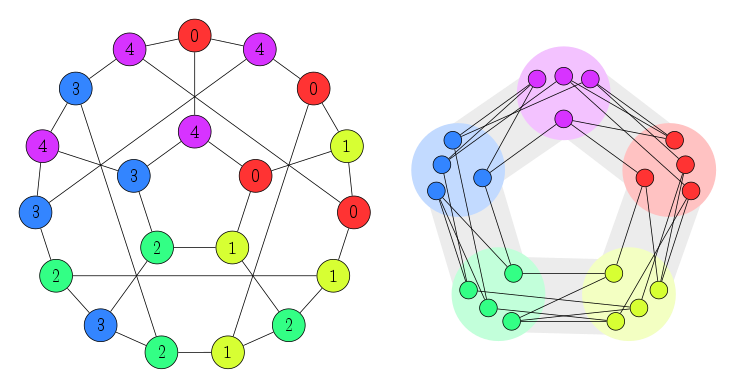
\includegraphics[width=\linewidth]{dismath/images/dismath_exam_list_graph_homomorphism}

                    Гомоморфизм

                    \smallvspace

                    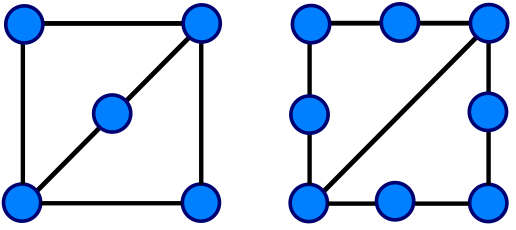
\includegraphics[width=\linewidth]{dismath/images/dismath_exam_list_graph_homeomorphism}

                    Гомеоморфизм
                \end{center}
            \end{wrapfigure}

            \smallvspace

            \item \textbf{Гомоморфизм графов} (\textit{Graph homomorphism})

            Гомоморфизм графов - отображение вершин графа $G$ в вершины графа $H$ такое,
            что смежные вершины графа $G$ отображаются в смежные вершины графа $H$


            \item \textbf{Гомеоморфизм графов} (\textit{Graph homeomorphism})

            Деление (Subdivision) ребра $\Pair{u, v}$ - операция, добавляющее верщину $w$, ребра $\Pair{u, w}$ и $\Pair{w, v}$ и удаляющее ребро $\Pair{u, v}$

            Исключение (Smoothing) вершины $w$ (степени 2) - операция, обратная делению - исключение вершины $w$ и ребер $\Pair{u, w}$ и $\Pair{w, v}$ и добавление ребра $\Pair{u, v}$

            Графы $G$ и $H$ гомеоморфны, если граф $H$ можно получить в результате деления или исключения графа $G$

        \end{minipage}

        \smallvspace

        \item \textbf{Пути и циклы} (\textit{Walks, paths, trails, cycles})

        Путь (Walk) - последовательность из вершин и ребер, соединяющих соседние вершины: $l = (v_0, e_0, v_1, e_1, \dots, e_{n - 1}, v_n)$

        Цепь (Trail) - путь (walk), все ребра которого различны

        Простая цепь (Path) - путь (walk), все вершины (и соответственно ребра) которого различны

        Замкнутый путь (Closed walk) - путь (walk), начальная вершина которого является конечной

        Контур (Circuit) - цепь (trail), являющаяся замкнутым

        Цикл (Cycle) - простая цепь (path), являющаяся замкнутым

        (*терминология из Википедии)


        \item \textbf{Эйлеровы путь, цикл, граф} (\textit{Eulerian path, cycle, graph})

        Эйлеров путь - путь, содержащий все ребра графа

        Эйлеров цикл - замкнутый путь, содержащий все ребра графа

        Граф называют эйлеровым, если в нем есть эйлеров цикл. Граф называют полуэйлеровым, если в ней есть эйлеров путь.

        \item \textbf{Теорема Эйлера для графов} (\textit{Euler's theorem for graphs})

        Граф эйлеров, если все степени вершин четные, а ребра принадлежат одной компоненте связности

        Граф полуэйлеров, если ровно 2 вершины имеют нечетную степень, а ребра принадлежат одной компоненте связности

        \item \textbf{Гамильтоновы путь, цикл, граф} (\textit{Hamiltonian path, cycle, graph})

        Гамильтонов путь - путь, содержащий все вершины графа

        Гамильтонов цикл - замкнутый путь, содержащий все вершины графа

        Граф называют гамильтоновым, если в нем есть гамильтонов цикл. Граф называют полугамильтоновым, если в ней есть гамильтонов путь.

        \item \textbf{Теорема Оре} (\textit{Ore’s theorem})

        Теорема Оре - достаточное условие существования гамильтонова цикла: если в графе $G(V, E)$ для любых $u, v \in V$ $\deg u + \deg v \geq |V|$, то граф $G$ гамильтонов

        \item \textbf{Теорема Дирака} (\textit{Dirac’s theorem})

        Теорема Дирака - достаточное условие существования гамильтонова цикла: если в графе $G(V, E)$ для любой $u \in V$ $\deg u \geq \frac{|V|}{2}$, то граф $G$ гамильтонов


        \item \textbf{Эксцентриситет вершины} (\textit{Eccentricity of a vertex})

        Расстояние $\text{dist}(u, v)$ - длина (количество ребер) кратчайшего пути между $u$ и $v$

        Эксцентриситет $\varepsilon(v)$ - наибольшая длина кратчайшего пути от этой вершины до другой в этом графе: $\varepsilon(v) = \max_{u \in V} \text{dist}(v, u)$

        \item \textbf{Радиус и диаметр графа} (\textit{Radius and diameter of a graph})

        Радиус графа $\text{rad}(G)$ - наименьший эксцентриситет вершины из графа: $\text{rad}(G) = \min_{v \in V} \varepsilon(v)$

        Диаметр графа $\text{diam}(G)$ - наибольший эксцентриситет вершины из графа: $\text{diam}(G) = \max_{v \in V} \varepsilon(v)$

        \item \textbf{Центр графа} (\textit{Center of a graph})

        Центр графа - вершина (вершины), эксцентриситет которой равен радиусу графа: $\text{center}(G) = \Set{v \in V \ | \ \varepsilon(v) = \text{rad}(G)}$

        \item \textbf{Центроид дерева} (\textit{Centroid of a tree})

        Центроид дерева - вершина (или 2 вершины), удаление которой приведет к распаду на поддеревья, каждое из которое имеет не больше $\frac{|V|}{2}$ вершин

        Очевидно, что только деревья, состоящие из четного количества вершин, могут иметь 2 центроида

        % TODO picture

        \item \textbf{Клика} (\textit{Clique})

        Клика графа - порожденный подграф, который является полный графом. $1$-клика - вершина, $2$-клика - 2 вершины и ребро, $3$-клика - треугольник, $n$-клика - граф $K_n$

        \item \textbf{Независимое (стабильное множество)} (\textit{Independent set})

        Независимое (стабильное) множество - множество вершин, каждая из которых не соединена ребром с другой вершиной из множества

        \item \textbf{Паросочетание} (\textit{Matching})

        Паросочетание (независимое множество ребер) - множество ребер, каждые из которые не соединяют одну и ту же вершину

        \item \textbf{Идеальное паросочетание} (\textit{Perfect matching})

        Идеальное паросочетание - паросочетание, ребра которого инцидентны ко всем вершинам графа (то есть паросочетание, являющееся реберным покрытием)

        \item \textbf{Вершинное покрытие} (\textit{Vertex cover})

        Вершинное покрытие - множество вершин, к которым инцидентны все ребра графа

        \item \textbf{Реберное покрытие} (\textit{Edge cover})

        Реберное покрытие - множество ребер, которые инцидентны ко всем вершинам

        \item \textbf{Дерево} (\textit{Tree})

        Дерево - связный ацикличный граф

        \item \textbf{Лес} (\textit{Forest})

        Лес - несвязный граф, каждая компонента которого не имеет циклов (граф, состоящий из деревьев)

        \item \textbf{Минимальное остовное дерево} (\textit{Minimum spanning tree})

        Минимальное остовное дерево взвешенного графа $G(V, E, w)$ - дерево $T(V, E^\prime)$, сумма весов ребер которого имеет наименьшее значение

        \item \textbf{Код Прюфера} (\textit{Prüfer code})

        Код Прюфера - алгоритм кодировки маркированного дерева размера $n$ в последовательность чисел

        \textbf{Кодировка}:

        1. Делаем биекцию между названиями вершин и числа из диапазона $[1;n]$ (если необходимо)

        2. Берем лист с наименьшим значением, удаляем его, записываем в последовательность номер его родителя

        3. Повторяем 2. до тех пор, пока не останется 2 вершины - их кодировка тривиальна и не нуждается в хранении

        \textbf{Декодировка}:

        1. Создаем $n$ вершин, и множество вершин $W$, которых нет в последовательности

        2. Читаем номер вершины из последовательности

        3. Соединяем эту вершину с вершиной из $W$ с минимальным номером, удалив ее

        4. Добавляем вершину из последовательности в $W$

        5. Повторяем 2.-4.

        6. Соединяем 2 оставшиеся вершины из $W$


        \item \textbf{Двудольный граф} (\textit{Bipartite graph})

        Двудольный граф $K_{n,m}$ - граф, вершины которого можно разбить на две части размеров $n$ и $m$ таким образом, что вершины из одной части не смежны друг с другом

        \item \textbf{Теорема баланса регулярных двудольных графов} (\textit{Theorem on the balance of regular bipartite graphs})

        Если двудольный граф $K_{n,m}$ регулярный, то $n = m$

        $\Box$ Граф регулярный $\Longrightarrow \forall v \in V \ \deg v = r \in \Natural \Longrightarrow $ левая доля имеет $nr$ исходящих ребер, а правая доля имеет $mr$ входящих ребер, но так как вершины в долях не соединены ребрами, $nr = mr$ $\Box$

        \item \textbf{Теорема существования идеального паросочетания регулярного двудольного графа} (\textit{Theorem on the existence of a perfect matching in a regular bipartite graph})

        Теорема: у любого $r$-регулярного двудольного графа ($r > 0$) существует идеальное паросочетание

        $\Box$

        Пусть $G(V, E)$ - граф, вершины разбиваются на две доли $X \xor Y = V$

        Пусть $N(A) = \Set{y \in Y \ | \ \exists x \in X \ \Pair{x, y} \in E}$ - соседи (смежные вершины) вершин из множества $A \subseteq X$

        Докажем от противного: пусть идеального паросочетания не существует, тогда по теореме Холла $\exists S \subset X \ | \ |S| > |N(S)|$,
        но тогда кол-во ребер, выходящих из $S$, равно $r|S|$, но кол-во ребер, выходящих из $N(S)$, равно $r|N(S)|$

        Из этого $r|S| > r|N(S)|$, что невозможно, так как $N(S)$ - соседи $S$ - противоречие

        $\Box$


        \item \textbf{Теорема Холла} (\textit{Hall's theorem (on the existence of an X-perfect matching in a bipartite graph)})

        Пусть $G(V, E)$ - граф, вершины разбиваются на две доли $X \xor Y = V$

        Тогда в графе $G(V, E)$ существует $X$-идеальное паросочетание (паросочетание, покрывающее все вершины $X$) тогда и только тогда,
        когда для любого $A \subset X \ |A| \leq |N(A)|$

        $\Box$ Если существует такое $A$, что $|A| > |N(A)|$, то какой-либо вершине из $A$ не найдется противоположная вершина из $N(A)$ и $X$-идеального паросочетания не выйдет $\Box$


        \item \textbf{Связность в неориентированных графах} (\textit{Connectivity in undirected graphs})

        Компонента связность графа - максимальный подграф, в котором от каждой вершины до любой другой существует путь

        Граф считается связным, если он представляет собой одну компоненту связности

        \item \textbf{Сильная и слабая связность в ориентированных графах} (\textit{Strong and weak connectivity in directed graphs})

        Компонента сильной связности - максимальный подграф, в котором для любых вершин $u, v$ существует пути $u \rightsquigarrow v$ и $v \rightsquigarrow u$

        Компонента слабой связности - максимальный подграф, который является компонентой связности в неориентированном графе, полученном при удалении ориентации ребер у исходного

        % TODO picture

        \item \textbf{Конденсация ориентированного графа} (\textit{Condensation of a directed graph})

        Конденсация графа - сжатие сильно связных компонент графа до вершин с целью получения упрощенного и ациклического графа

        \item \textbf{Вершинная связность} (\textit{Vertex connectivity})

        Вершинная связность $\kappa(G)$ графа $G$ - минимальное число вершин, которое нужно удалить в графе, чтобы он стал несвязным или синглтоном

        \item \textbf{Реберная связность} (\textit{Edge connectivity})

        Реберная связность $\lambda(G)$ графа $G$ - минимальное число ребер, которое нужно удалить в графе, чтобы он стал несвязным

        \item \textbf{Теорема Уитни} (\textit{Whitney's theorem})

        Для любого графа $\kappa(G) \leq \lambda(G) \leq \delta(G)$

        $\Box$

        Допустим, что $\kappa(G) > \lambda(G)$, тогда после удаления $\lambda(G)$ ребер будет $k \leq \lambda(G)$ вершин со одной стороны и $m \leq \lambda(G)$ с другой.
        Но мы их тоже можем удалить, и граф распадется, значит $\lambda < \kappa(G) = \min (k, m) \leq \lambda(G)$ - противоречие

        Допустим, что $\lambda(G) > \delta(G)$, тогда мы можем найти в графе вершину с наименьшей степенью $\delta(G)$,
        при удалении $\delta(G)$ ребер граф распадется, значит $\lambda(G) = \delta(G)$ - противоречие

        $\Box$


        \item \textbf{$k$-связный граф} (\textit{k-connected graph})

        $k$-вершинно-связный граф - граф, остающийся связным после удаления $k$ вершин ($\kappa(G) \geq k$).

        НО: синглтон имеет $\kappa(G) = 0$, он не $1$-вершинно-связный, при этом он связный; $K_2$ имеет $\kappa(G) = 1$,
        поэтому он не $2$-вершинно-связный, но $K_2$ может быть блоком

        $k$-реберно-связный граф - граф, остающийся связным после удаления $k$ ребер ($\lambda(G) \geq k$)

        НО: у синглтона $\lambda(G) = 0$, он не $1$-реберно-связный, при этом синглтон - компонента реберной двусвязности

        \item \textbf{Теорема Менгера} (\textit{Menger's theorem})

        Теорема (Менгера о реберной двойственности в ориентированном графе):

        Между вершинами $u$ и $v$ существует $L$ реберно непересекающихся путей тогда и только тогда,
        когда после удаления любых $(L - 1)$ ребер существует путь из $u$ в $v$.

        Теорема (Менгера о вершинной двойственности в ориентированном графе):

        Между вершинами $u$ и $v$ существует $L$ вершинно непересекающихся путей тогда и только тогда,
        когда после удаления любых $(L - 1)$ вершин существует путь из $u$ в $v$.

        \href{https://neerc.ifmo.ru/wiki/index.php?title=%D0%A2%D0%B5%D0%BE%D1%80%D0%B5%D0%BC%D0%B0_%D0%9C%D0%B5%D0%BD%D0%B3%D0%B5%D1%80%D0%B0#.D0.A2.D0.B5.D0.BE.D1.80.D0.B5.D0.BC.D0.B0}{Доказательства}


        \item \textbf{Двусвязность} (\textit{Biconnectivity})

        Двусвязность (вершинная) определяется как отношение эквивалентности 2 ребер, между концами которых существуют 2 вершинно-различных пути  % a little strange

        Компонента (вершинной) двусвязности (также блок) - подграф, который включает все двусвязные ребра (класс эквивалентности двусвязности).

        Реберная двусвязность определяется как отношение эквивалентности 2 вершины, между которыми существуют 2 реберно-различных пути

        Компонента реберной двусвязности - подграф, который включает все двусвязные вершины (класс эквивалентности двусвязности).

        \item \textbf{Точка сочленения} (\textit{Articulation point})

        Точка сочленения - вершина, принадлежащая нескольким компонентам (вершинной) двусвязности

        \item \textbf{Мост} (\textit{Bridge})

        Мост - ребро, соединяющее две компоненты реберной двусвязности

        \item \textbf{Блок} (\textit{Blocks})

        Блок - компонента вершинной двусвязности

        \item \textbf{Дерево блоков и точек сочленений} (\textit{Block-cut tree})

        Дерево блоков и точек сочленений графа - дерево, в котором каждая вершина представляет собой либо точку сочленения, либо блок,
        при этом вершина точки сочленения соединена только с вершиной блока и наоборот

        % TODO bc-tree picture

    \end{enumerate}

    \begin{center}
        \textbf{6. Теория автоматов.}
    \end{center}


    \begin{enumerate}
        \item \textbf{Детерминированный конечный автомат} (\textit{Deterministic Finite Automaton (DFA)})

        Детерминированный конечный автомат $A = (Q, \Sigma, \delta, q_0, F)$ - объект, представляющий собой множество состояний $Q$, множество входных символов $\Sigma$,
        функция переходов $\delta \ : \ Q \times \Sigma \to Q$, начальное состояние $q_0$ и множество конечных состояний $F$

        Автомат принимает какую-то цепочку символов из $\Sigma^*$ и решает, принадлежит ли она соответствующему автомату регулярному языку $L$

        Для простоты обычно выбирают $\Sigma = \Set{0, 1}$

        Автомат можно представить как орграф

        \tikz[myautomatonstyle]{
            \node[state, initial] (s0) {$q_0$};
            \node[below=0.75cm of s0] (s0cc) {начальное};
            \node[state, right=3cm of s0] (s1) {$q_2$};
            \node[state, accepting, right=3cm of s1] (s2) {$q_1$};
            \node[below=0.75cm of s2] (s0cc) {конечное};
            \path[->]
            (s0) edge [above] node {$0$} (s1)
            (s0) edge [loop above, above] node {$1$} (s0)
            (s1) edge [above] node {$1$} (s2)
            (s1) edge [loop above, above] node {$0$} (s1)
            (s2) edge [loop above, above] node {$0,1$} (s2)
            ;
        }

        Или как таблицу функции переходов

        \begin{tabular}{c|cc}
            & $0$   & $1$   \\
            \hline
            $\to q_0$ & $q_2$ & $q_0$ \\
            \hline
            $*q_1$    & $q_1$ & $q_1$ \\
            \hline
            $q_2$     & $q_2$ & $q_1$
        \end{tabular}

        \item \textbf{Недетерминированный конечный автомат (НКА)} (\textit{Non-deterministic Finite Automaton (NFA)})

        Недетерминированный конечный автомат $A = (Q, \Sigma, \delta, q_0, F)$ - объект, представляющий собой множество состояний $Q$, множество входных символов $\Sigma$,
        функция переходов $\delta \ : \ P(Q) \times \Sigma \to \mathcal{P}(Q)$, начальное состояние $q_0$ и множество конечных состояний $F$

        Главное отличие НКА от ДКА: от одного состояния в НКА можно перейти сразу к нескольким другим или к ни одному

        Пример:

        \begin{multicols}{2}
            \tikz[myautomatonstyle]{
                \node[state, initial] (s0) {$q_0$};
                \node[state, right=3cm of s0] (s1) {$q_1$};
                \node[state, accepting, right=3cm of s1] (s2) {$q_2$};
                \path[->]
                (s0) edge [loop above, above] node {$0,1$} (s0)
                (s0) edge [above] node {$0$} (s1)
                (s1) edge [above] node {$1$} (s2)
                ;
            }

            \begin{tabular}{c|cc}
                & $0$              & $1$         \\
                \hline
                $\to q_0$ & $\Set{q_0, q_1}$ & $\Set{q_0}$ \\
                \hline
                $q_1$     & $\emptyset$      & $\Set{q_1}$ \\
                \hline
                $*q_2$    & $\emptyset$      & $\emptyset$
            \end{tabular}

        \end{multicols}

        \item \textbf{Формальные языки} (\textit{Formal languages})

        Формальный язык $L$ - множество конечных слов над конечным алфавитом символов $\Sigma$

        \item \textbf{Операции над формальными языками (конкатенация, объединение, замыкание Клини)} (\textit{Operations on formal languages (concat, union, Kleene closure)})

        Конкатенация $LM$ языков $L$ и $M$ - множество слов, состоящих из записанных подряд слова из $L$ и слова из $M$: $LM = \Set{uw \ | \ u \in L \land w \in M}$

        Объединения $L \union M$ языков $L$ и $M$ - множество слов, которые содержатся в $L$ или/и в $M$: $L \union M = \Set{w \ | \ w \in L \lor w \in M}$

        Замыкание Клини $L^*$ языка $L$ - множество слов, которые могут быть получены в результате конкатенации слов из $L$: $L^* = \Set{w_1 w_2 \dots w_n \forall n \geq 0 \ | \ w_i \in L}$ (включая пустое слово $\varepsilon$)

        \item \textbf{Регулярные языки} (\textit{Regular languages})

        Регулярный язык - формальный язык, который задается некоторым автоматом

        Также регулярный язык задается индуктивно:

        1. Пустое множество $\emptyset$ и множество из пустой строки $\Set{\varepsilon}$ являются регулярными языками

        2. Множество из однобуквенного слова $\Set{a}$, где $a \in \Sigma$ является регулярным языком

        3. Для регулярных языков $\alpha$ и $\beta$ объединение $\alpha \union \beta$, конкатенация $\alpha\beta$ и замыкание Клини $\alpha^*$ - тоже регулярные языки

        4. Других регулярных языков нет

        \item \textbf{Регулярное выражение} (\textit{Regular expression})

        Регулярное выражение - способ описания регулярного языка

        \begin{tabular}{c|c}
            Регулярное выражение & Язык, который оно описывает \\
            \hline
            & $\emptyset$                 \\
            $\varepsilon$        & $\Set{\varepsilon}$         \\
            $a$ (какое-либо РВ)  & $\alpha$                    \\
            $b$ (какое-либо РВ)  & $\beta$                     \\
            $(a)$                & $\alpha$                    \\
            $ab$                 & $\alpha\beta$               \\
            $a + b$              & $\alpha \union \beta$       \\
            $a*$                 & $\alpha^*$                  \\

        \end{tabular}

        \item \textbf{Теорема Клини} (\textit{Kleene's theorem})

        Для любого регулярного выражения существует конечный автомат, и они описывают равные регулярные языки

        \item \textbf{Конструкция подмножеств (ДКА из НКА)} (\textit{Powerset construction (DFA from NFA)})

        Из состояний $Q$ НКА построим ДКА с состояниями, каждое из которых представляет собой подмножество $Q$.
        Далее при помощи магии умным образом строим переходы

        \begin{multicols}{2}
            \tikz[myautomatonstyle]{
                \node[state, initial] (s0) {$q_0$};
                \node[state, right=2cm of s0] (s1) {$q_1$};
                \node[state, accepting, right=2cm of s1] (s2) {$q_2$};
                \path[->]
                (s0) edge [loop above, above] node {$0,1$} (s0)
                (s0) edge [above] node {$0$} (s1)
                (s1) edge [above] node {$1$} (s2)
                ;
            }

            \smallvspace

            \begin{tabular}{c|cc}
                & $0$              & $1$              \\
                \hline
                $\emptyset$            & $\emptyset$      & $\emptyset$      \\
                \hline
                $\to\Set{q_0}$         & $\Set{q_0, q_1}$ & $\Set{q_0}$      \\
                \hline
                $\Set{q_1}$            & $\emptyset$      & $\Set{q_2}$      \\
                \hline
                $\Set{q_0, q_1}$       & $\Set{q_0, q_1}$ & $\Set{q_0, q_2}$ \\
                \hline
                $*\Set{q_2}$           & $\emptyset$      & $\emptyset$      \\
                \hline
                $*\Set{q_2, q_0}$      & $\Set{q_0, q_1}$ & $\Set{q_0}$      \\
                \hline
                $*\Set{q_2, q_1}$      & $\emptyset$      & $\Set{q_2}$      \\
                \hline
                $*\Set{q_2, q_1, q_0}$ & $\Set{q_0, q_1}$ & $\Set{q_0, q_2}$ \\
            \end{tabular}

            \tikz[myautomatonstyle]{
                \node[state, initial] (s0) {\scriptsize $\Set{q_0}$};
                \node[state, right=2cm of s0] (s01) {\scriptsize $\Set{q_0, q_1}$};
                \node[state, accepting, right=2cm of s01] (s02) {\scriptsize $\Set{q_0, q_2}$};
                \node[state, accepting, right=2cm of s02] (s012) {\scriptsize $\Set{q_0, q_1, q_2}$};
                \node[state, below=2cm of s0] (s) {\scriptsize $\emptyset$};
                \node[state, right=2cm of s] (s1) {\scriptsize $\Set{q_1}$};
                \node[state, accepting, right=2cm of s1] (s2) {\scriptsize $\Set{q_2}$};
                \node[state, accepting, right=2cm of s2] (s12) {\scriptsize $\Set{q_1, q_2}$};
                \path[->]
                (s) edge [loop left, left] node {$0,1$} (s)
                (s0) edge [loop above, above] node {$1$} (s0)
                (s0) edge [above] node {$0$} (s01)
                (s1) edge [above] node {$1$} (s2)
                (s1) edge [above] node {$0$} (s)
                (s01) edge [loop above,above] node {$0$} (s01)
                (s01) edge [bend left,above] node {$1$} (s02)
                (s02) edge [bend left,below] node {$0$} (s01)
                (s02) edge [out=-135,in=-45,above] node {$1$} (s0)
                (s012) edge [out=135,in=45,above] node {$0$} (s01)
                (s012) edge [above] node {$1$} (s02)
                (s12) edge [above] node {$1$} (s2)
                (s12) edge [out=-135,in=-45, below] node {$0$} (s)
                (s2) edge [out=-135,in=-45, above] node {$0,1$} (s)
                ;
            }
        \end{multicols}

        Как можем видеть, 5 состояний являются недостижимыми, поэтому их мы можем удалить.
        В итоге в ДКА остается 3 состояния (зачастую количество состояний не $2^{|Q|}$, а чуть больше $|Q|$)

        \tikz[myautomatonstyle]{
            \node[state, initial] (s0) {\scriptsize $\Set{q_0}$};
            \node[state, right=2cm of s0] (s01) {\scriptsize $\Set{q_0, q_1}$};
            \node[state, accepting, right=2cm of s01] (s02) {\scriptsize $\Set{q_0, q_2}$};
            \path[->]
            (s0) edge [loop above, above] node {$1$} (s0)
            (s0) edge [above] node {$0$} (s01)
            (s01) edge [loop above,above] node {$0$} (s01)
            (s01) edge [bend left,above] node {$1$} (s02)
            (s02) edge [bend left,below] node {$0$} (s01)
            (s02) edge [out=-135,in=-45,below] node {$1$} (s0)
            ;
        }

        \item \textbf{$\varepsilon$-НКА} (\textit{$\varepsilon$-NFA})

        $\varepsilon$-НКА $A = (Q, \Sigma, \delta, q_0, F)$ - НКА, допускающий $\varepsilon$ переходы (переходы по пустым строчкам)
        Тогда $\delta \ : \ Q \times (\Sigma \union \Set{\varepsilon}) \to \mathcal{P}(Q)$

        Пример - автомат, допускающий цепочки $(01)*$:

        \tikz[myautomatonstyle]{
            \node[state, initial] (s0) {$q_0$};
            \node[state, right=2cm of s0] (s1) {$q_1$};
            \node[state, accepting, right=2cm of s1] (s2) {$q_2$};
            \path[->]
            (s0) edge [above] node {$0$} (s1)
            (s1) edge [above] node {$1$} (s2)
            (s2) edge [out=-135,in=-45,below] node {$\varepsilon$} (s0)
            ;
        }

        \item \textbf{Конструкция НКА из $\varepsilon$-НКА} (\textit{NFA construction from $\varepsilon$-NFA})

        Алгоритм:

        1. Транзитивное замыкание: если из состояния $u$ мы можем сделать больше одного $\varepsilon$-перехода в состояние $w$, то мы можем сделать сразу $\varepsilon$-переход из $u$ в $w$

        2. Добавление допускающих состояний: если есть $\varepsilon$-переход из $u$ в $w$, причем $w$ - допускающее состояние, то $u$ можно сделать тоже допускающем

        3. Добавление ребер: если есть переходы $\delta(u, \varepsilon) = v$ и $\delta(v, c) = w$, то сделаем равное ребро $\delta(u, c) = w$

        4. Удаление $\varepsilon$-переходов

        \item \textbf{Конструкция Томпсона ($\varepsilon$-НКА из регулярного выражения)} (\textit{Thompson’s construction ($\varepsilon$-NFA from regular expression)})


        \begin{tabular}{m{0.12\linewidth}|m{0.12\linewidth}|m{0.76\linewidth}}
            Регулярное выражение & Язык, который оно описывает & Автомат \\
            \hline

            & $\emptyset$ & \smallvspace \tikz[myautomatonstyle]{
                \node[state, initial] (s0) {};
            } \\
            $\varepsilon$ & $\Set{\varepsilon}$ & \tikz[myautomatonstyle]{
                \node[state, initial] (s0) {};
                \node[state, accepting, right=2cm of s0] (s1) {};
                \path[->] (s0) edge [above] node {$\varepsilon$} (s1);
            } \\
            $c$ (символ) & $\Set{c}$ & \tikz[myautomatonstyle]{
                \node[state, initial] (s0) {};
                \node[state, accepting, right=2cm of s0] (s1) {};
                \path[->] (s0) edge [above] node {$c$} (s1);
            } \\
            $ab$ & $\alpha\beta$ & \tikz[myautomatonstyle]{
                \node[state, initial] (s0) {};
                % \node[above right=2cm and 2cm of s0] (r1) [draw, rounded rectangle] {rectangle \\ oppopoopo};
                \node[state, right=1.5cm of s0] (r1) {};
                \node[right=1.5cm of r1] (rcap) {Автомат $\alpha$};
                \node[state, right=3cm of r1] (r2) {};
                \node[state, right=1.5cm of r2] (l1) {};
                \node[right=1.5cm of l1] (lcap) {Автомат $\beta$};
                \node[state, right=3cm of l1] (l2) {};
                \node[state, accepting, right=1.5cm of l2] (s1) {};
                \draw[rounded corners] ([xshift=-0.1cm,yshift=-0.5cm]r1.west) rectangle ([xshift=0.1cm,yshift=0.5cm]r2.east) {};
                \draw[rounded corners] ([xshift=-0.1cm,yshift=-0.5cm]l1.west) rectangle ([xshift=0.1cm,yshift=0.5cm]l2.east) {};
                \path[->]
                (s0) edge [bend left, above] node {$\varepsilon$} (r1)
                (r2) edge [bend right, above] node {$\varepsilon$} (l1)
                (l2) edge [bend left, above] node {$\varepsilon$} (s1)
                ;
            } \\
            $a + b$ & $\alpha \union \beta$ & \tikz[myautomatonstyle]{
                \node[state, initial] (s0) {};
                % \node[above right=2cm and 2cm of s0] (r1) [draw, rounded rectangle] {rectangle \\ oppopoopo};
                \node[state, above right=0.65cm and 2cm of s0] (r1) {};
                \node[right=1.5cm of r1] (rcap) {Автомат $\alpha$};
                \node[state, right=3cm of r1] (r2) {};
                \node[state, below right=0.65cm and 2cm of s0] (l1) {};
                \node[right=1.5cm of l1] (lcap) {Автомат $\beta$};
                \node[state, right=3cm of l1] (l2) {};
                \node[state, accepting, right=7cm of s0] (s1) {};
                \draw[rounded corners] ([xshift=-0.1cm,yshift=-0.5cm]r1.west) rectangle ([xshift=0.1cm,yshift=0.5cm]r2.east) {};
                \draw[rounded corners] ([xshift=-0.1cm,yshift=-0.5cm]l1.west) rectangle ([xshift=0.1cm,yshift=0.5cm]l2.east) {};
                \path[->]
                (s0) edge [bend left, above] node {$\varepsilon$} (r1)
                edge [bend right, above] node {$\varepsilon$} (l1)
                (l2) edge [bend right, above] node {$\varepsilon$} (s1)
                (r2) edge [bend left, above] node {$\varepsilon$} (s1)

            } \\
            $a*$ & $\alpha^*$ & \tikz[myautomatonstyle]{
                \node[state, initial] (s0) {};
                \node[state, above right=1cm and 2cm of s0] (r1) {};
                \node[right=1.5cm of r1] (rcap) {Автомат $\alpha$};
                \node[state, right=3cm of r1] (r2) {};
                \node[state, accepting, right=7cm of s0] (s1) {};
                \draw[rounded corners] ([xshift=-0.1cm,yshift=-0.5cm]r1.west) rectangle ([xshift=0.1cm,yshift=0.5cm]r2.east) {};
                \path[->]
                (s0) edge [bend left, above] node {$\varepsilon$} (r1)
                edge [bend right, below] node {$\varepsilon$} (s1)
                (r2) edge [bend left, above] node {$\varepsilon$} (s1)
                ;
                \draw[->] (r2) edge [out=-130,in=-50,below] node {$\varepsilon$} (r1)
            } \\


        \end{tabular}

        Пользуясь этими преобразованиям, можно построить $\varepsilon$-НКА


        \item \textbf{Алгоритм Клини} (\textit{Kleene’s algorithm})

        Алгоритм Клини - алгоритм для превращения ДКА в регулярное выражение

        Пусть ДКА $(Q, \Sigma, \delta, q_0, F)$, а $Q = \Set{q_0, \dots, q_n}$, $F = \Set{q_i \ | \ i \in \Natural_F \subset \Natural}$

        Определим $R^{-1}_{ij} = a_1 + \dots + a_m$, где $q_j \in \delta(q_i, a_k)$ для $k$ - другими словами все символы, по которым можно перейти из $q_i$ в $q_j$.
        Для $i = j$ $R^{-1}_{ii} = a_1 + \dots + a_m + \varepsilon$

        Далее для каждого $k$ от $0$ до $n$ итеративно определяем

        $R^k_{ij} = R^{k - 1}_{ik} (R^{k - 1}_{kk})* R^{k-1}_{kj} | R^{k-1}_{ij}$

        Таким образом, ответом будет регулярное выражение $\bigunion_{i \in \Natural_F} R^n_{0i}$

        \item \textbf{Лемма о накачке для регулярных языков} (\textit{Pumping lemma for regular languages})

        Если $L$ - регулярный язык, то существует константа $p \geq 1$, зависящая от $L$, такая, что любая строка $w \in L (|w| \geq p)$
        может быть записана $w = xyz$ так, что удовлетворены условия:

        1. $|y| \geq 1$

        2. $|xy| \leq p$

        3. Для любого $n \geq 0$ $xy^n z \in L$

        \item \textbf{Свойства замыкания регулярных языков} (\textit{Closure properties of regular languages})

        Для регулярных языков $L$ и $M$:

        1. $L^*$ (замыкание Клини) - регулярный язык

        2. $L \union M$ (объединение) - регулярный язык

        3. $LM$ (конкатенация) - регулярный язык

        4. $L \cap M$ (пересечение) - регулярный язык

        5. $\overline{L}$ (дополнение - $\Sigma^* \setminus L = \overline{L}$) - регулярный язык

        6. $L^R$ (инверсия - $abac \to caba$) - регулярный язык

        7. $L \setminus M$ (разность) - регулярный язык

        8. $h(L)$ (гомоморфизм $h \ | \ \Sigma \to \Sigma^*$, например $h(0) = ab, h(1) = ba$) - регулярный язык

        9. $h^{-1}(L)$ (обратный гомоморфизм $h^{-1} \ | \ \Sigma^* \to \Sigma$, например $h^{-1}(01) = a, h^{-1}(10) = b$) - регулярный язык

        \smallvspace

        \begin{minipage}{\linewidth}
            \begin{wrapfigure}{R}{0.4\linewidth}
                \tikz[myautomatonstyle]{
                    \node[state, initial] (s0) {$q_0$};
                    \node[state, right=2cm of s0] (s1) {$q_1$};
                    \node[state, right=2cm of s1] (s2) {$q_2$};
                    \path[->]
                    (s0) edge [bend left, above] node {$0/0$} (s1)
                    (s0) edge [bend right, below] node {$1/1$} (s1)
                    (s1) edge [bend left, above] node {$0/0$} (s2)
                    (s1) edge [bend right, below] node {$1/1$} (s2)
                    (s2) edge [out=-130,in=-50, below] node {$0/1$} (s0)
                    (s2) edge [out=130,in=50, above] node {$1/0$} (s0)
                    ;
                }

                \footnotesize
                \textit{Этот автомат Мили преобразует каждый 3-ий символ с 0 на 1 и наоборот:} $\mathtt{100101} \to \mathtt{101100}$

            \end{wrapfigure}

            \item \textbf{Автомат Мили} (\textit{Mealy machine})

            Автомат Мили $M_{\text{Mealy}} = (Q, \Sigma, \Omega, q_0, \delta, \lambda)$ - автомат, выводящий последовательность, которая зависит от входной последовательности

            Здесь $\Omega$ - алфавит выходящей последовательности, а
            $\lambda \ : \ Q \times \Sigma \to \Omega$ - функция выходов, зависящая от состояния и входного символа

            Значение функции $\lambda$ на ребре графа обозначают после переходного символа


        \end{minipage}

        \begin{minipage}{\linewidth}
            \begin{wrapfigure}{R}{0.35\linewidth}
                \tikz[myautomatonstyle]{
                    \node[state, initial] (s0) {$q_0/${\Large 👍}};
                    \node[state, right=2cm of s0] (s1) {$q_1/${\Large 💀}};
                    \node[state, right=2cm of s1] (s2) {$q_2/${\Large 💀}};
                    \path[->]
                    (s0) edge [loop above, above] node {$0$} (s0)
                    (s0) edge [bend left, above] node {$1$} (s1)
                    (s1) edge [bend left, above] node {$0$} (s2)
                    (s1) edge [bend left, below] node {$1$} (s0)
                    (s2) edge [bend left, below] node {$0$} (s1)
                    (s2) edge [loop above, above] node {$1$} (s0)
                    ;
                }

                \footnotesize
                \textit{Этот автомат Мура выдает {\Large 👍}, если двоичное число делится на 3, иначе {\Large 💀}}


            \end{wrapfigure}

            \item \textbf{Автомат Мура} (\textit{Moore machine})

            Автомат Мура $M_{\text{Moore}} = (Q, \Sigma, \Omega, q_0, \delta, \lambda)$ - автомат, выводящий последовательность, зависящую от входной последовательности

            Как и в автомате Мили, в автомате Мура $\Omega$ - алфавит выходящей последовательности, но
            $\lambda \ : \ Q \to \Omega$ - функция выходов, зависящая от текущего состояния

            Значение функции $\lambda$ на графе обозначают в вершине состояния

        \end{minipage}

        \smallvspace


        \item \textbf{Пустота языка конечного автомата} (\textit{Emptiness of finite automaton language})

        Язык автомата $L$ считается пустым в том случае, если язык не содержит никаких цепочек (в том числе пустых) - $L = \emptyset$

        По конечному автомату можно понять, является ли язык пустым: если какое-либо допускающее состояние можно достигнуть из начального,
        то язык автомата не является пустым (это можно определить при помощи обхода графа)

        \item \textbf{Конечность языка конечного автомата} (\textit{Finiteness of finite automaton language})

        Язык автомата $L$ считается конечным, если он содержит конечное множество цепочек

        Конечность языка можно определить так: если есть такое состояние $v$, что к нему можно прийти из начального состояния,
        от него можно прийти к какому-либо допускающему состоянию, а из $v$ можно каким-либо образом прийти в $v$, то язык бесконечный -
        мы можем сколь угодно раз зацикливаться по $v$ и получать бесконечное количество цепочек

        \item \textbf{Эквивалентность конечных автоматов} (\textit{Equivalence of finite automata})

        Автоматы эквивалентны, если они допускают одно и то же множество цепочек.

        Пусть автомат $A = (Q, \Sigma, \delta, q_0, F)$. Введем функцию $\lambda \ : \ Q \to \Set{0, 1}$, возвращающую $\mathtt{1}$, если состояние допускающее, иначе $\mathtt{0}$

        Введем такое отношение эквивалентности $R_0 \subset Q \times Q$ между состояниями. Определим, что $q \, R_0 \, p$ в том случае, если $\lambda(q) = \lambda(p)$

        Теперь определим $R_1$ как отношение состояний $q$ и $p$, для которых $\lambda(q) = \lambda(p)$ и $\lambda(\delta(q, c)) = \lambda(\delta(p, c))$ для любого символа $c \in \Sigma$

        Теперь определим $R_2$ как отношение состояний $q$ и $p$, для которых $\lambda(\hat\delta(q, w)) = \lambda(\hat\delta(p, w))$ для любой цепочки $w \in \Sigma^*$ длины не больше 2

        Окончательно определим $R$ как отношение состояний $q$ и $p$, для которых $\lambda(\hat\delta(q, w)) = \lambda(\hat\delta(p, w))$ для любой цепочки $w \in \Sigma^*$


        \begin{minipage}{\linewidth}
            \begin{wrapfigure}{R}{0.35\linewidth}
                \tikz[myautomatonstyle]{
                    \node[state, initial] (m0) {$q_1$};
                    \node[state, accepting, right=3.5cm of m0] (m1) {$F_1$};
                    \node[right=0.1cm of m0.east] (mcap) {Автомат $M$};
                    \draw[rounded corners] ([xshift=-0.3cm,yshift=-0.6cm]m0.west) rectangle
                        ([xshift=0.3cm,yshift=0.6cm]m1.east) {};


                    \node[state, below=2cm of m0] (n0) {$q_2$};
                    \node[state, accepting, right=3.5cm of n0] (n1) {$F_2$};
                    \node[right=0.1cm of n0.east] (ncap) {Автомат $N$};
                    \draw[rounded corners] ([xshift=-0.3cm,yshift=-0.6cm]n0.west) rectangle
                        ([xshift=0.3cm,yshift=0.6cm]n1.east) {};

                    \node[below right=0.3cm and 0.5cm of n0.south] (acap) {Автомат $A$};
                    \draw[rounded corners] ([xshift=-0.6cm,yshift=-1.6cm]n0.west) rectangle
                        ([xshift=0.6cm,yshift=1.2cm]m1.east) {};
                }

            \end{wrapfigure}

            Пусть даны автоматы $M = (Q_1, \Sigma, \delta_1, q_1, F_1)$ и $N = (Q_2, \Sigma, \delta_2, q_2, F_2)$.

            Теперь построим такой автомат $A = (Q, \Sigma, \delta, q_1, F)$, выбрав какое-либо начальное состояние, объединив множества состояний и множества допускающих состояний и расширив функцию переходов

            Автоматы $M$ и $N$ эквивалентны, если состояния $q_1$ и $q_2$ принадлежат одному классу эквивалентности, то есть $q_1 \, R \, q_2$

        \end{minipage}

        \smallvspace

        \item \textbf{} (\textit{Myhill-Nerode theorem})

    \end{enumerate}


    \begin{center}
        \textbf{7. Комбинаторика.}
    \end{center}


    \begin{enumerate}
        \item \textbf{} (\textit{Ordered arrangements})

        \item \textbf{} (\textit{Permutations})

        \item \textbf{} (\textit{k-permutations})

        \item \textbf{} (\textit{Cyclic permutations})

        \item \textbf{} (\textit{Unordered arrangements})

        \item \textbf{} (\textit{k-combinations})

        \item \textbf{} (\textit{Multisets})

        \item \textbf{} (\textit{Permutations of multisets})

        \item \textbf{} (\textit{Combinations of infinite multisets})

        \item \textbf{} (\textit{Compositions})

        \item \textbf{} (\textit{Set partitions})

        \item \textbf{} (\textit{Stirling numbers of the second kind})

        \item \textbf{} (\textit{Integer partitions})

        \item \textbf{} (\textit{Principle of Inclusion-Exclusion})

    \end{enumerate}

    \begin{center}
        \textbf{8. Рекуррентности и производящие функции.}
    \end{center}


    \begin{enumerate}
        \item \textbf{} (\textit{Recurrence relations})

        \item \textbf{} (\textit{Solving recurrence relations using characteristic equations})

        \item \textbf{} (\textit{Generating functions})

        \item \textbf{} (\textit{Power series})

        \item \textbf{} (\textit{Solving linear recurrences using generating functions})

        \item \textbf{} (\textit{Solving combinatorial problems using generating functions})

        \item \textbf{} (\textit{Operators and annihilators})

        \item \textbf{} (\textit{Solving linear recurrences using annihilators})

        \item \textbf{} (\textit{Catalan numbers})

        \item \textbf{} (\textit{Divide-and-Conquer algorithms analysis using recursion trees})

        \item \textbf{} (\textit{Master theorem})

        \item \textbf{} (\textit{Akra-Bazzi method})

    \end{enumerate}
    % end dismath_exam_list.tex



\end{document}

